\documentclass{article}

%packages
\usepackage{graphicx}
\usepackage{tikz}
\usepackage[utf8]{inputenc}
\usepackage{amssymb}

\usepackage[T1]{fontenc}
\usepackage{mathabx}
\def\MCr{
	\multicolumn{1}{c}{
		\rule{-5pt}{0ex}$\stackrel{}{\curvearrowleft}$
		\rule{+20pt}{0ex}$\stackrel{}{\curvearrowright}$
	}
}
\def\MCe{\multicolumn{1}{c}{}}

\begin{document}

\usetikzlibrary{automata,arrows, positioning}
\renewcommand{\contentsname}{Tabla de contenidos}

\begin{titlepage}
	\begin{center}
		
\includegraphics{./images/escudo.jpg}
	\end{center}
	\centering
	{\scshape\LARGE Complutense de Madrid \par}
	\vspace{1cm}
	{\scshape\Large Práctica Programación Evolutiva.\par}
	\vspace{1.5cm}
	{\huge\bfseries Tercera práctica. \par}
	\vspace{2cm}
	{\Large\itshape Raúl Torrijos \& Lukas Häring\par}
	%{\large Grupo 9\par}
	\vfill
	\vfill

% Bottom of the page
	{\large \today\par}
\end{titlepage}

\tableofcontents

\newpage
\section{Introducción}
En está versión hemos implementado una modificación del Algoritmo Genético en la que utilizamos cromosomas en forma de árbol para buscar una solución al problema de la Hormiga sobre el Rastro de Santa Fe, usando como función de evaluación el número de alimentos devorados por la hormiga sobre el tablero siguiendo las instrucciones de un programa generado de manera evolutiva.

\subsection{Algoritmos implementados}
Los algoritmos de selección, cruce y mutación que hemos utilizado para la resolución del problema de la hormiga son:


\begin{enumerate}
	\item Algoritmos de Selección
		\begin{itemize}
			\item Selección por Ruleta
			\item Selección por Torneo Determinista
			\item Selección por Torneo Probabilista
			\item Selección por Ranking
			\item Selección por Truncamiento
		\end{itemize}
	\item Algoritmos de Cruce
		\begin{itemize}
			\item Método Subárboles
		\end{itemize}
	\item Algoritmos de Mutación
		\begin{itemize}
			\item Terminal Simple
			\item Funcional Simple
			\item Subárbol
			\item Permutación (no accesible en la interfaz)
		\end{itemize}
	\item Mejoras adicionales al guión
		\begin{itemize}
			\item Pestaña de visualización de árboles
		\end{itemize}
\end{enumerate}
\newpage
\subsection{Aclaraciones}
Nos gustaría puntualizar un par de pequeñas decisiones que hemos tomado a la hora de implementar el ejercicio:\par
\bigskip
\quad- Hemos decidido eliminar todas las tildes de la interfaz de la aplicación por un motivo de problemas con nuestro software de control de versiones.\par En cualquier caso nuestra implementación está preparada para ejecutar el problema con más o menos ciudades.\par
\bigskip
\quad- La manera en la que controlamos el bloating es un con una operación que penaliza el fitness de un programa restando al número de alimentos devorados por la hormiga el tamaño del árbol en cuestión por un factor K, que hemos establecido en 0.5. Esto evita la aparición de árboles muy grandes. \par Es por esto que con el control de bloating activado, el fitness de ciertos individuos se puede ver afectado por su tamaño y en la pestaña de gráficas puede no coincidir el máximo absoluto con el número de alimentos comidos en realidad. \par Hemos hecho pruebas con el control de bloating desactivado y los árboles que genera son demasiado grandes.

\newpage
\section{Paneles de resultados}

\subsection{Gráficas}
Idéntico al de las prácticas anteriores. Puede no reflejar resultados fieles a la cantidad de alimentos comidos por la hormiga si tenemos el control de bloating activo.
\subsection{Pestaña Mapa}
Nuestra aplicación incorpora una visualización del tablero toroidal de 32x32 con rastro de alimento en color negro, y tras ejecutar el AG mostrará la ejecución del mejor programa absoluto sobre el tablero, mostrando en color naranja el alimento devorado por la hormiga, y en color azul el recorrido de la hormiga realizado fuera del Rastro.\par También se muestra la posición final de la hormiga tras representada con un cuadrado rojo con ojos negros, que indican la posición donde mira.

\subsection{Pestaña Mejor Árbol}
Como ya hicimos en la Práctica 2, hemos querido añadir un pequeño extra y en está ocasión hemos adjuntado una pestaña con un panel que, de igual manera, muestra el mejor resultado tras ejecutar el algoritmo y muestra el árbol de manera gráfica.\par Esta característica nos fué extremadamente útil a la hora de comprobar que los algoritmos de cruce y mutación funcionaban correctamente.\par
Hemos usado la libreria org.abego.treelayout (https://github.com/abego/treelayout) para generar el árbol en Java Swing. \par  

\begin{figure}[h]
	\centering
	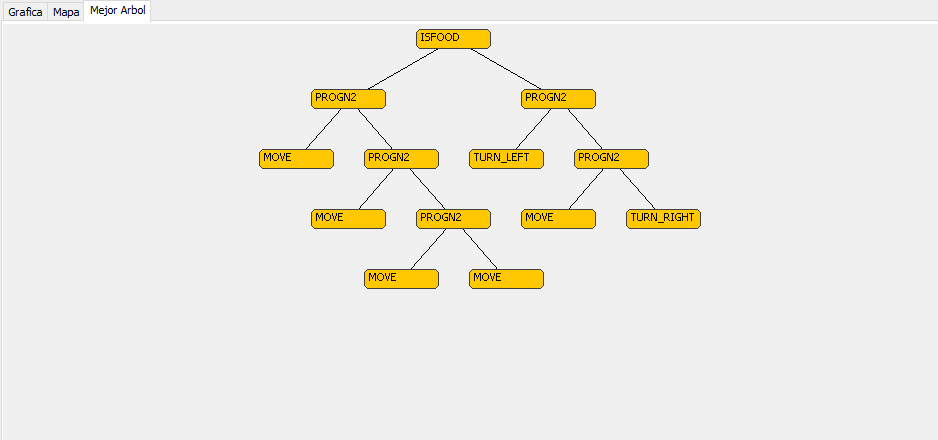
\includegraphics[scale=0.4]{./images/marbol.png}
	\caption{Pestaña de Mejor Árbol}
\end{figure}

\newpage
\section{Análisis de ejecuciones}
Para realizar un análisis exhaustivo del comportamiento de cada uno de los algoritmos usados hemos realizado una gran cantidad de ejecuciones y hemos obtenido las siguientes conclusiones.
\subsection{Peores resultados}

De nuevo el método de selección de ruleta es el que menos favorece a la evolución por gran componente aleatoria.\par 
Un número menor a 300 en el número de generaciones puede no ser suficiente para evolucionar de manera correcta por encima de los >70 alimentos comidos.\par La contractividad en este experimento juega un mal papel ya que de por sí tenemos unos algoritmos muy costosos (gran cantidad de accesos a memoria) y no hace mejorar el proceso.


\\
\begin{figure}[h]
	\centering
	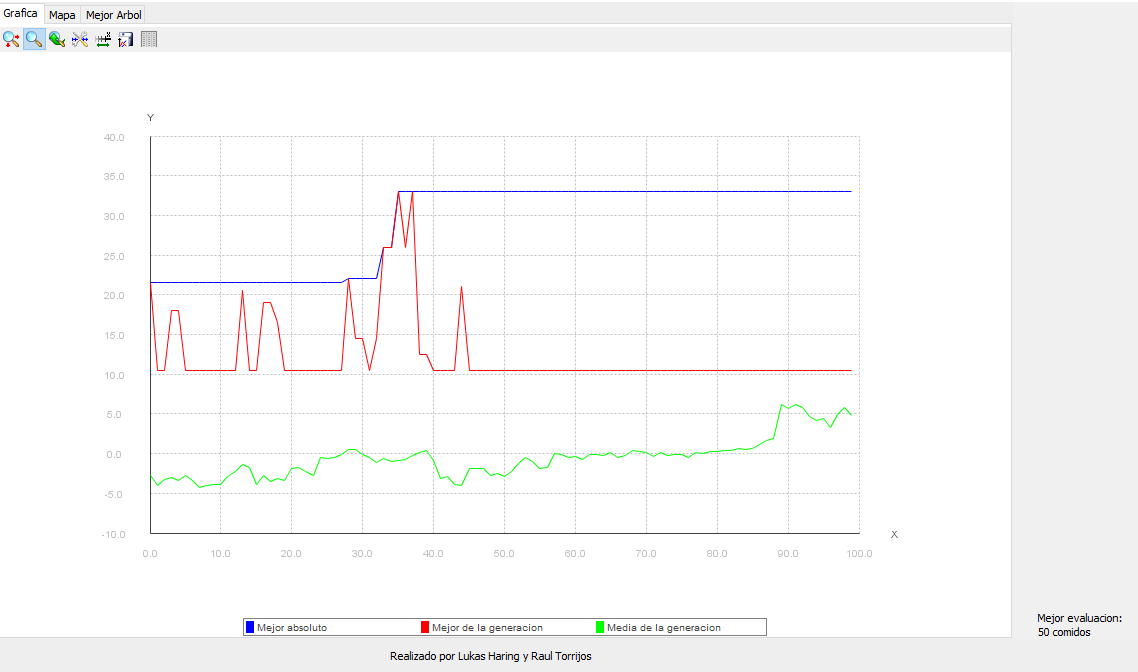
\includegraphics[scale=0.4]{./images/3rul1.png}
	\caption{Ruleta sin elitismo (50 alimentos)}
\end{figure}

La única manera de obtener resultados mas razonables utilizando ruleta es aumentando el número de generaciones y usar elitismo para así aumentar la variedad en la población.
\begin{figure}[h]
	\centering
	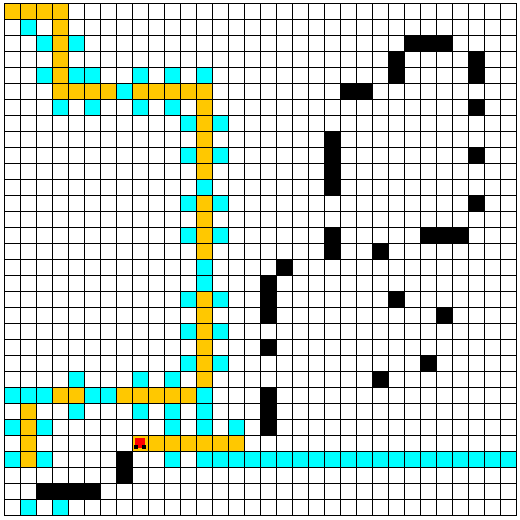
\includegraphics[scale=0.5]{./images/3rul2.png}
	\caption{Ruleta sin elitismo (50 alimentos)}
\end{figure}

\newpage
\newpage
\subsection{Mejores resultados}
Los mejores resultados que hemos obtenido han sido aumentando el tamaño de población a 400, usando selección mediante Torneo Determinista o Ranking y mutación y cruce mediante subárboles.\par
En 10 ejecuciones hemos obtenido 4 veces el que consideramos el valor máximo \textbf{solución: 90 (o 89) alimentos}(esto es porque consideramos que en la posición inicial la hormiga come 1 alimento). \par También nos ha ayudado mucho aumentar los valores de probabilidad de mutación y cruce hasta valores de 0.3 y 0.7~0.8 respectivamente y elitismo con valor 5.
\par Es importante que exista variedad en la población de individuos para aumentar la probabilidad de que se genere un programa que recorra el Rastro completo.
\begin{figure}[h]
	\centering
	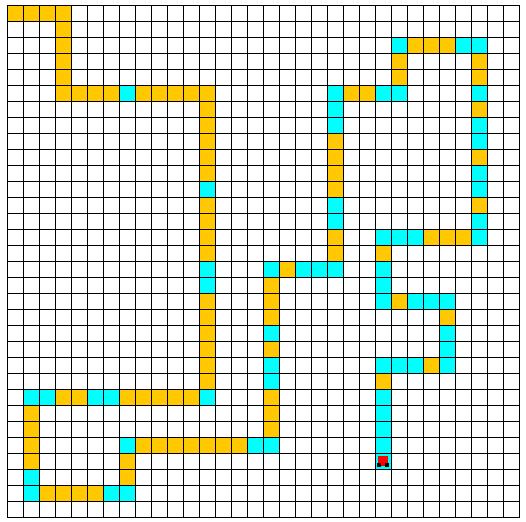
\includegraphics[scale=0.35]{./images/3fin1.png}
	\caption{Representación en el tablero. Mejor resultado obtenido. 90 alimentos}
\end{figure}

\begin{figure}[h]
	\centering
	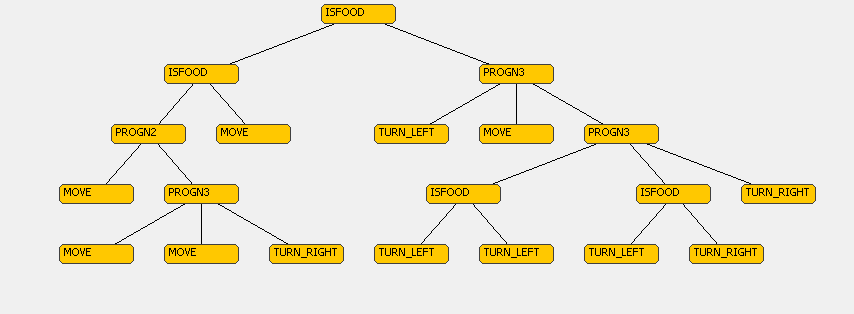
\includegraphics[scale=0.35]{./images/3fin2.png}
	\caption{Grafo del mejor cromosoma.}
\end{figure}

\begin{figure}[h]
	\centering
	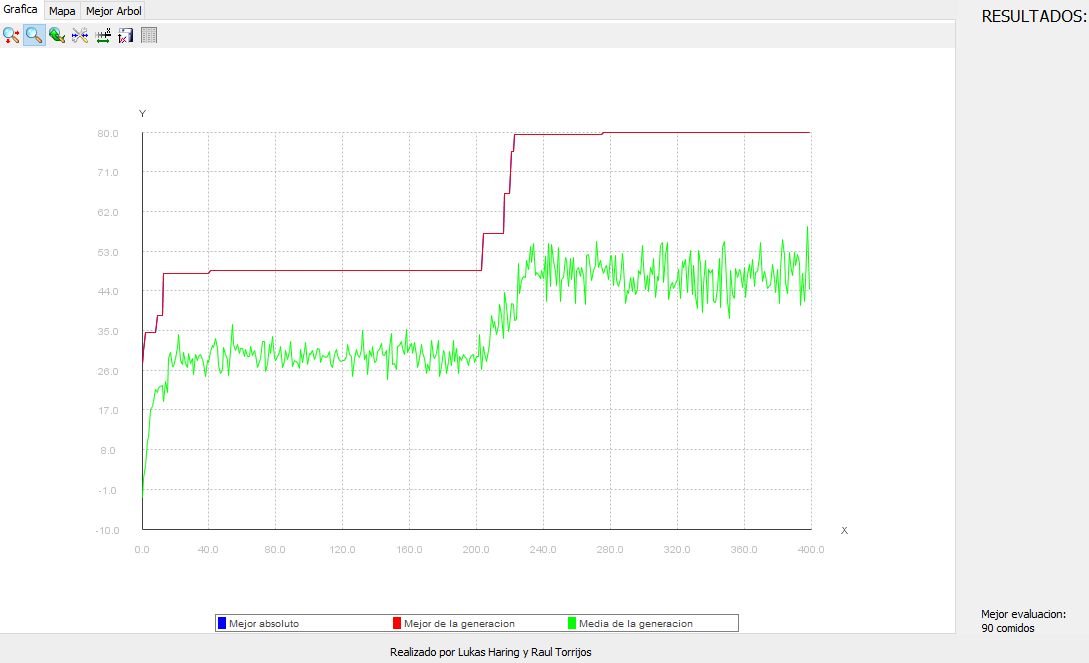
\includegraphics[scale=0.35]{./images/3fin3.png}
	\caption{Gráficas de evolución.}
\end{figure}
\end{document}
